
% ---------------------------------------- Major Branches of Deep Learning -------------------------
\section{Major Branches of Deep Learning}
\subsection{Supervised Learning}
Supervised learning is one of the most widely used branches of deep learning. It involves training models on datasets where each input is paired with a corresponding output, commonly referred to as a \textit{label}. This approach enables models to learn the relationship between inputs and their known results, allowing them to make accurate predictions on new, unseen data. In essence, supervised learning is like teaching a system through examples where the correct answers are already provided.
Supervised learning tasks typically fall into two categories:
\begin{itemize}
\item \textit{Classification:} Sorting data into predefined categories. For example, classifying land cover types (e.g., forests, urban areas, water bodies) based on satellite images.
\item \textit{Regression:} Predicting continuous numerical values. An example is forecasting river water levels based on historical data and environmental conditions.
\end{itemize}
Supervised learning () plays a pivotal role in hydrology and environmental sciences, powering a wide range of applications such as image classification, temperature forecasting, and hurricane tracking. To tackle these tasks, specific deep learning architectures are particularly effective. For example, Recurrent Neural Networks (RNNs) and their advanced variant, Long Short-Term Memory networks (LSTMs), excel at processing and forecasting sequential data, making them ideal for analyzing time-series datasets like rainfall records or river flow patterns. On the other hand, Convolutional Neural Networks (CNNs) are exceptionally adept at handling image-based tasks. They are commonly used for interpreting satellite images, such as identifying land cover types or detecting environmental changes.
Here are some representative examples of how supervised learning is applied in hydrology and environmental sciences:
\begin{itemize}
    \item \textit{Precipitation Forecasting:} Predicting rainfall amounts to aid in water resource management and flood prevention.
\item \textit{Drought Severity Classification:} Determining the severity of droughts to assist in agricultural planning and water conservation.
\item \textit{Land Cover Classification:} Categorizing earth surface types (e.g., forests, croplands, urban areas) from satellite imagery for applications like urban planning and ecosystem monitoring.
\item \textit{Image Segmentation:} Identifying specific regions in satellite images, such as flood-affected areas, deforested zones, or crop health conditions.
\item \textit{Object Detection:} Identifying and categorizing objects in satellite imagery, such as water bodies, vegetation types, or urban areas.
\end{itemize}


\begin{figure}[h!]
    \centering
    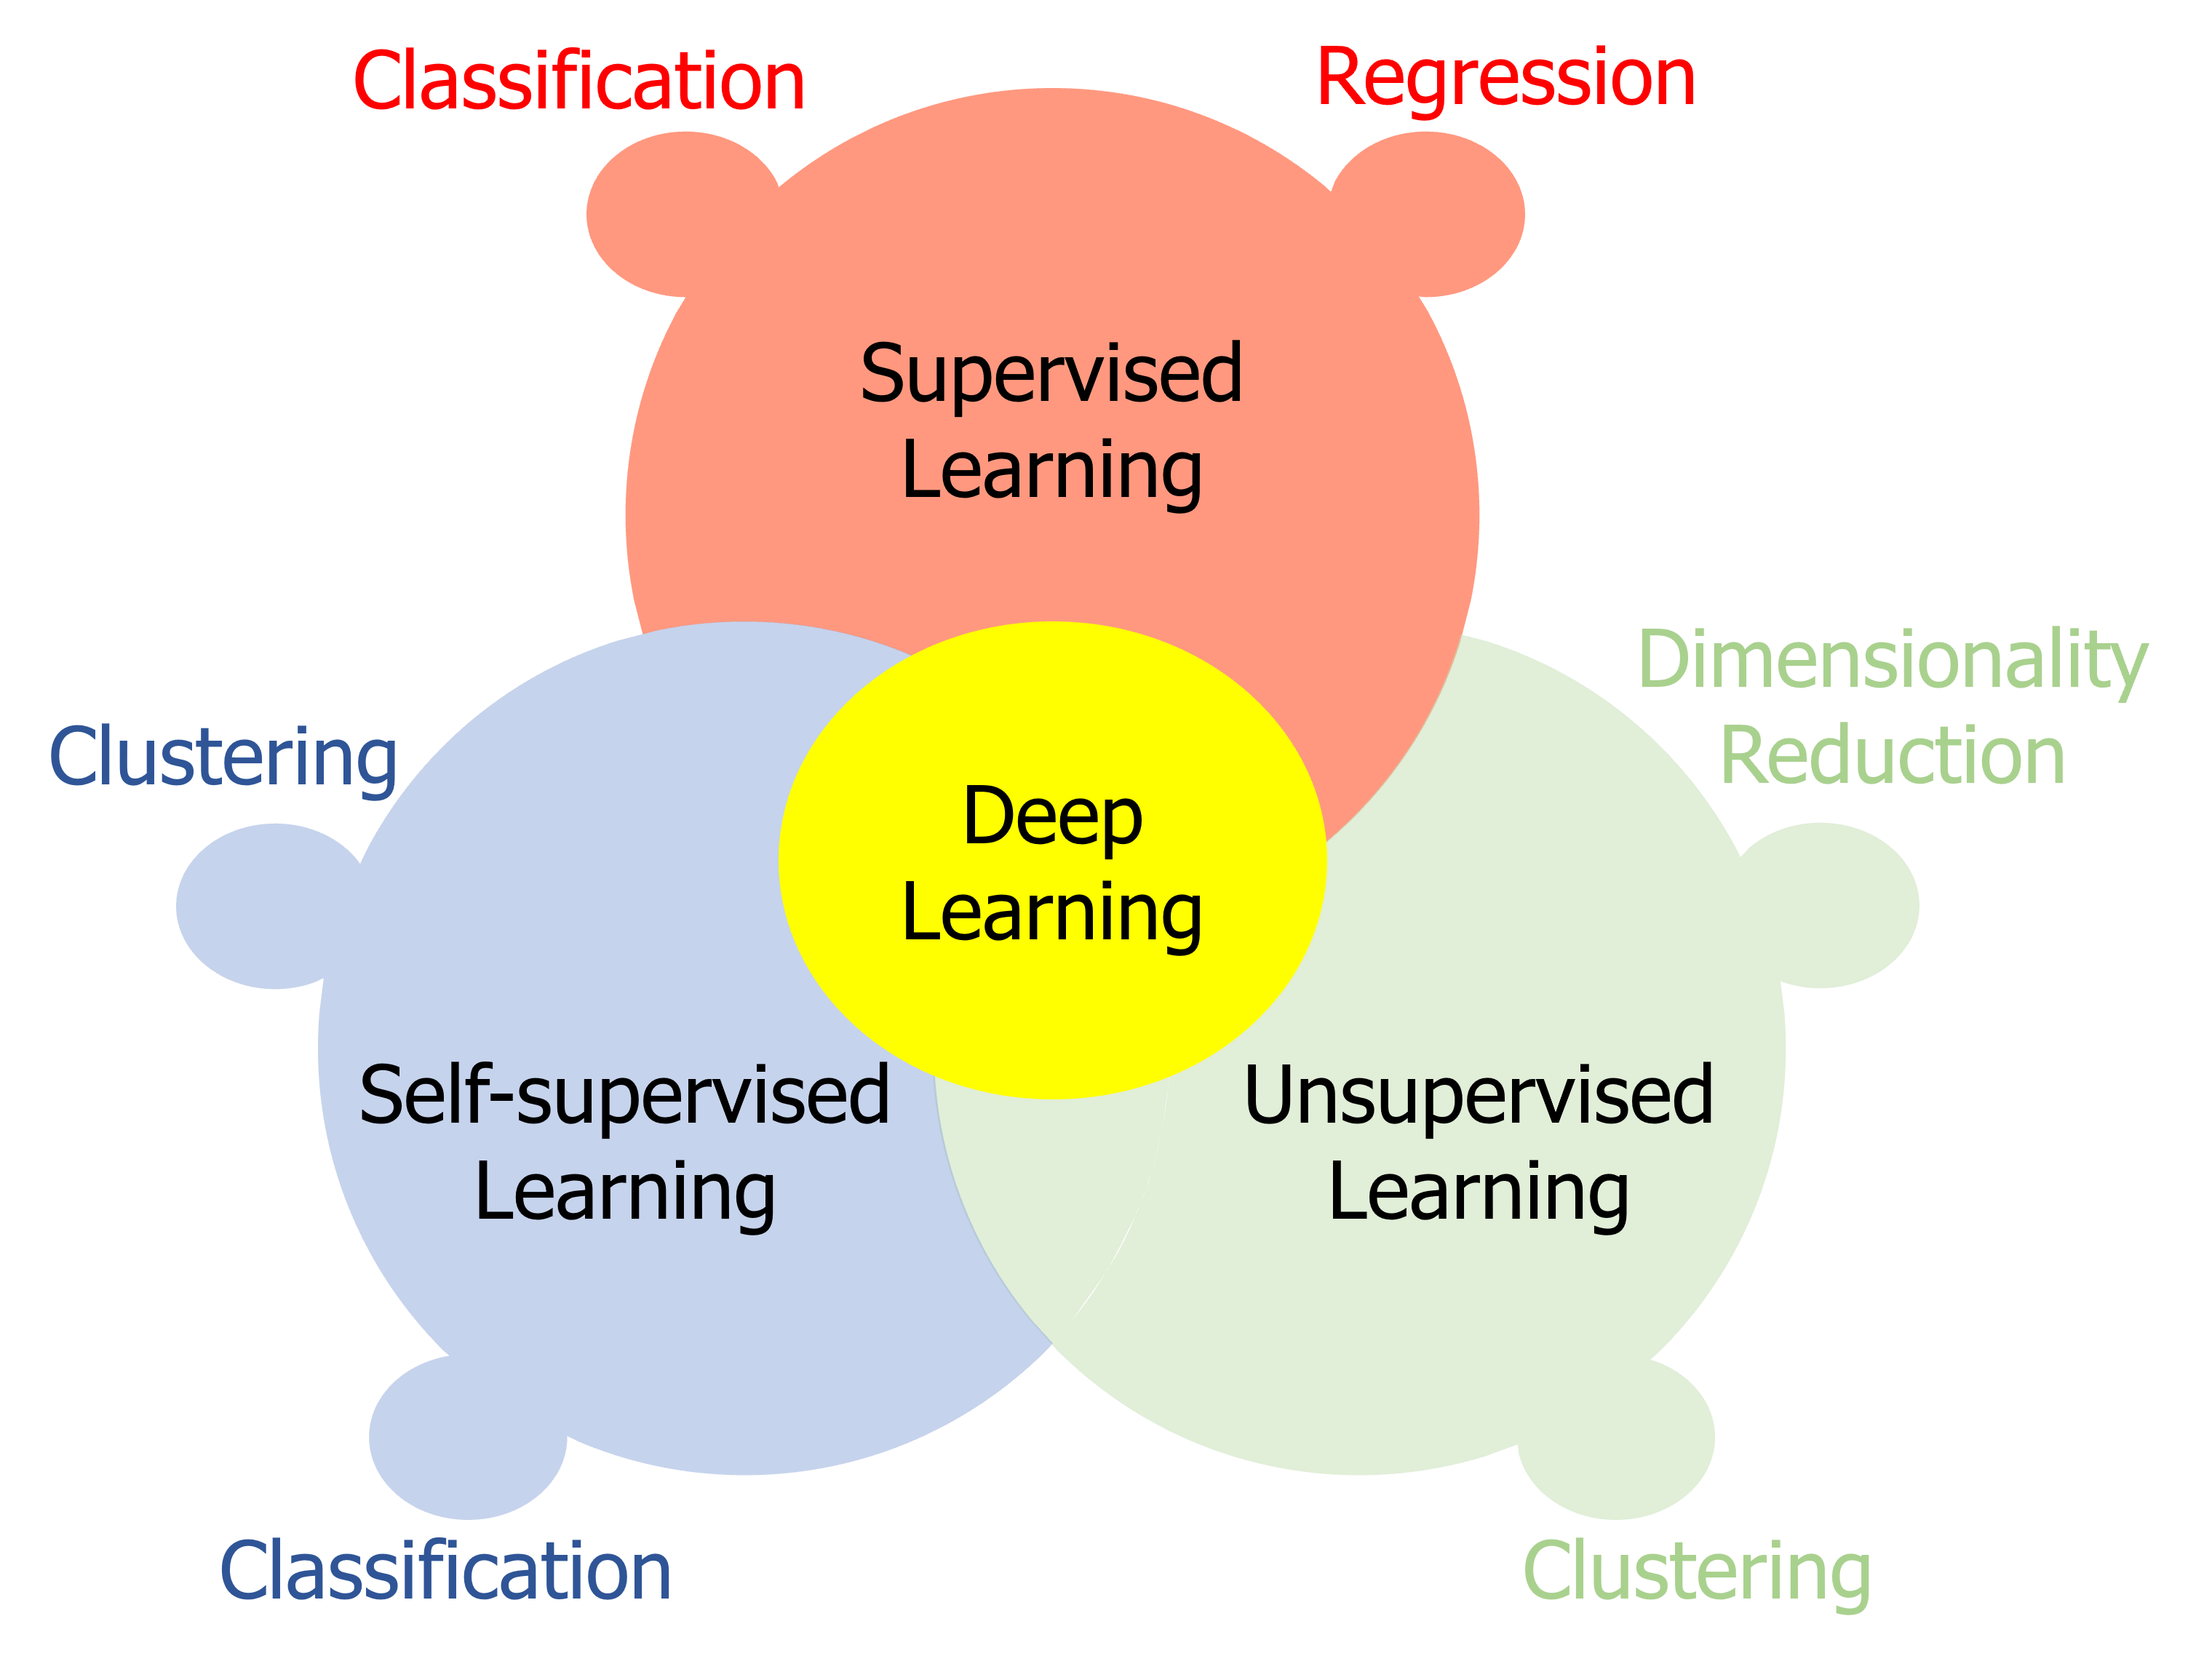
\includegraphics[width=\linewidth]{images/supervised_learning_classification_image.png}
    \caption{Three Major branches of Deep Learning: supervised learning, unsupervised learning, and self-supervised learning.}
    \label{fig:supervised}
\end{figure}


\subsection{Unsupervised Learning }

Unsupervised learning focuses on uncovering patterns, structures, and transformations within data, all without relying on labeled outputs. Instead of predicting a specific target, it aims to reveal insights such as correlations, clusters, or low-dimensional representations. This type of learning is invaluable in hydrology and environmental sciences, where complex datasets often need to be distilled into more interpretable or actionable forms. 
Unsupervised learning is foundational for tasks like data visualization, where the goal is to represent high-dimensional data in an intuitive way, and dimensionality reduction, which simplifies large datasets while retaining essential information. It also plays a critical role in data denoising, improving the quality of noisy remote sensing data to make subsequent analyses more reliable. Before solving supervised learning problems, unsupervised learning can act as a crucial first step to explore and understand the dataset, identify outliers, and discover hidden relationships.

\begin{itemize}
    \item \textit{Data Visualization:} Creating intuitive visual representations of high-dimensional datasets, such as water quality measurements spanning multiple variables, to better understand spatial and temporal trends.
    \item \textit{Dimensionality Reduction:} Simplifying vast climatic datasets, like global temperature records or precipitation grids, for faster processing and storage while preserving critical patterns.
    \item \textit{Data Denoising:} Enhancing the quality of noisy remote sensing data (e.g., satellite imagery or LiDAR scans) to improve the accuracy of downstream analyses like land cover classification or flood mapping.
    \item \textit{Clustering:} Identifying groups in the data, such as categorizing regions based on similar hydrological characteristics or climate patterns, without pre-defined labels.

\end{itemize}


\subsection{Self-Supervised Learning}

Self-supervised learning is a DL approach where the model generates its own labels directly from the input data, removing the need for human-annotated labels. These pseudo-labels guide the learning process, making it possible to utilize large amounts of unlabeled data. This is particularly beneficial in hydrology, where labeled datasets are often limited or incomplete.

A key advantage of self-supervised learning is its scalability. By automatically generating pseudo-labels, it avoids the time and cost associated with manual labeling. A well-known example of self-supervised learning is the autoencoder, a model that compresses data into a compact representation (the "encoder") and then reconstructs it back to its original form (the "decoder"). The reconstruction error—the difference between the input and the reconstructed output—provides the learning signal. We will explore autoencoders in detail in Chapter~\ref{chap:acn} with a practical example.

Here are two simple examples to illustrate self-supervised learning:

\begin{itemize}
    \item \textit{Noise Removal in Satellite Images:} Autoencoders can clean noisy satellite images by learning to reconstruct meaningful features, such as water boundaries, while removing noise.
    \item \textit{Predicting Missing Data:} Models can predict missing streamflow values based on surrounding data, helping to fill gaps in hydrological records for further analysis.
\end{itemize}

\textbf{NOTE:} In this book, we’ll primarily focus on supervised learning, as it remains the most widely used and impactful form of deep learning in hydrology and environmental sciences, powering applications like precipitation forecasting, flood mapping, and drought prediction. We’ll also briefly explore self-supervised learning in later chapters, as it offers promising solutions for leveraging large, unlabeled datasets, which are common in these fields.

\subsection{Reinforcement Learning (RL)}
There is another branch of DL called Reinforcement Learning (RL), where an agent interacts with its environment, learning through trial and error to take actions that maximize a reward signal. Unlike traditional DL, which focuses on mapping inputs to outputs, RL emphasizes decision-making in dynamic environments. For example, an RL model could determine optimal reservoir release strategies by balancing flood control and water conservation. While RL has shown success in fields like robotics and gaming, its applications in hydrology are still largely in the research phase. In this book, we will primarily focus on supervised learning, leaving RL for further exploration in advanced studies.

% ----------------------------------------Evaluating Deep Learning Models -------------------------



























